\section{Simulation Datasets} \label{app:dataset}
%
This section provides detailed information about the datasets used in our experiments. 
%
The key characteristics of each dataset are summarized in Table~\ref{tab:dataset_description}. \texttt{Deforming Block} and \texttt{Sheet Deformation} consist of $16$ simulation trials per task with various initial conditions, \texttt{Trampoline} and \texttt{Bending Beam} consist of $10$ simulation trials per task.
%
\begin{table}[h]
\centering
\caption{Dataset descriptions}
\label{tab:dataset_description}
\begin{tabular}{lccc}
\toprule
Name & Train/Val/Test Splits & Number of Steps & Number of Nodes \\
\midrule
Deforming Block       & 600/100/100   & 52  & 81 \\
Sheet Deformation & 460/50/50 & 50  &  225 \\
Bending Beam & 380/60/60 & 100 & ~180 \\
Trampoline  & 600/100/100 & 25  &  ~1700 \\
\bottomrule
\end{tabular}
\end{table}
%


\subsection{Trampoline.}
%
% \texttt{Trampoline (Sim)} consists of a \texttt{2D} deformable membrane clamped by a rigid frame and deformed by a spherical impactor of varying size and density falling under gravity.
% The membranes follow a nearly incompressible viscoelastic material model, with Young's modulus $E$ sampled uniformly from $[1,5]$ MPa, Poisson's ratio fixed to $\nu=0.499$, membrane thickness $t$ uniformly from $[0.15,0.4]$ mm, shear relaxation ratio $g$ uniformly from $[0.01,0.3]$, and relaxation time $\tau$ log-uniformly from $[10^{-2},10^{1}]$ s.
% The dataset includes $600/100/100$ train/val/test tasks with $10$ trajectories of $25$ steps each. Each scene contains roughly $1700$ nodes and $3300$ triangular elements.
% 
This dataset models a thin square deformable sheet clamped by a rigid frame and deformed by a spherical impactor of varying size and density falling under gravity. Rigid body motion prediction of the ball is enforced by predicting per-node velocities and averaging them across all ball nodes
The sheet has initial stress-free edge length $l_{\textrm{init}}=245$~mm.
The sheet is discretized by $9604$ triangular membrane elements and $4901$ nodes, with membrane thickness $t$ varied as described below. 
To emulate the rigid frame in the physical setup, the sheet is pre-stretched to an edge length of $l=260$~mm by applying Dirichlet boundary conditions along its outer boundary.
%
\par
%
Data generation follows a two-stage sampling procedure. 
%
In the first stage, a simulation configuration is defined by sampling the sheet material parameters together with the properties of a rigid spherical impacter. 
%
The sheet material is modeled as a nearly incompressible viscoelastic solid with rubber-like behavior. 
%
The instantaneous Young's modulus is sampled uniformly from $E \in [1,5]$~MPa, the Poisson's ratio is fixed to $\nu=0.499$, and the membrane thickness is sampled from $t \in [0.15,0.4]$~mm. 
%
Rate dependence is modeled using a single-term Prony series with shear relaxation ratio $g \in [0.01,0.3]$ and relaxation time $\tau \in [10^{-2},10^{1}]$~s.
%
Volumetric relaxation is neglected ($k=0$). 
%
The impacter diameter is chosen from $15$ to $55$~mm in steps of $5$~mm, with each diameter represented by a pre-meshed geometry of approximately $1000$ elements. 
%
Its mass is sampled from $[0.009,0.269]$~kg, subject to density bounds between $268$~kg/m$^3$ (3D-printed PLA with $10\%$ infill) and $7850$~kg/m$^3$ (steel).
%
Gravitational loading is applied as an equivalent concentrated force at the impacter's center of mass. 
%
\par
%
In the second stage, $10$ trajectories are generated for each fixed stage-one configuration by varying only the initial conditions of the spherical impacter. 
%
Specifically, the in-plane drop position is sampled from a Gaussian distribution centered at the sheet origin and truncated to $[-75,75]$~mm in each in-plane direction, while the drop height is sampled within $[120,280]$~mm.
%
Contact between the impacter and the sheet is modeled using hard normal contact to prevent interpenetration. 
%
Tangential contact is governed by a Coulomb friction law with coefficient $\mu=0.7$. 
%
All simulations are performed in \textsc{Abaqus/Explicit} using explicit time integration.

%
\subsection{Bending Beam.}
%
% \texttt{Bending Beam} consists of $2$D beams clamped on the left side that bend and deform over time due to external forces applied on the right side. 
% The beams follow an isotropic Kelvin--Voigt viscoelastic material model, with Young's modulus $E$ sampled log-uniformly from $[0.5, 5.0]$, Poisson's ratio $\nu$ uniformly from $[0.0, 0.45]$, and viscosity $\tau$ log-uniformly from $[0.05, 0.5]$.
% The dataset includes $380/60/60$ train/val/test tasks with $10$ trajectories of $100$ steps each.
%
This scene consists of $2$D beams clamped on the left side that bend and deform over time due to time-varying external forces applied on the right side.
%
The beam is modeled as a rectangular domain embedded in two dimensional space.
%
The left boundary of the beam is clamped with zero displacement, while external forces are applied to the right boundary.
%
The load consists of one horizontal and one vertical force component.
%
The horizontal force magnitude is sampled uniformly in $[-1.0{\cdot}10^{-7}, 1.0{\cdot}10^{-7}]$, while the vertical force magnitude is sampled uniformly in $[-3.0{\cdot}10^{-5}, 3.0{\cdot}10^{-5}]$.
%
The forces are varied smoothly over time using cubic spline interpolation, starting from zero force, reaching the sampled target magnitude, and returning to zero before the end of the simulation.
%
The beam height is sampled normally with mean $0.3$ and standard deviation $0.01$, and the beam length is sampled normally with mean $10.0$ and standard deviation $1.0$.
%
The maximum characteristic mesh length, used for mesh generation, is sampled normally with mean $0.2$ and standard deviation $0.02$.
%
The material behavior is modeled using an isotropic Kelvin--Voigt viscoelastic material model, combining an elastic stress response with a viscous stress contribution.
%
Young's modulus $E$ is sampled log-uniformly in $[0.5, 5.0]$, Poisson's ratio $\nu$ is sampled uniformly in $[0.0, 0.45]$, and the viscosity parameter $\tau$ is sampled log-uniformly in $[0.05, 0.5]$.
%
Geometric non-linearities due to large deformations are considered.
%
The beam is discretized using linear triangular elements.
%
The simulations are implemented in \texttt{scikit-fem} and solved using Newton iterations with a residual tolerance of $10^{-8}$.
%
We create a total of $500$ simulations, each consisting of $40{,}000$ time steps. For the \gls{gns}, we subsample to $100$ time steps per trajectory.
%

\subsection{Deforming Block.}
%
% \texttt{Deforming Block} consists of $2$D trapezoids deformed by a circular collider.
% The material varies by Poisson's ratio, which is sampled uniformly from $[-0.9, 0.49]$.
% The dataset contains $600/100/100$ train/val/test tasks, each with $16$ trajectories of $52$ simulation steps.
% \texttt{Deforming Block} consists of $2$D trapezoids with Poisson's ratios uniformly sampled from $[-0.9, 0.49]$ that are deformed by a circular collider. 
% The dataset for this environment contains $600/100/100$ train/val/test tasks, each containing $16$ trajectories of $52$ simulation steps.
%
This scene consists of $2$D trapezoids deformed by a circular collider. 
%
This environment was originally implemented by \citet{linkerhagner2023grounding} and uses \gls{sofa} \citep{faure2012sofa}. 
%
This dataset considers the deformation of a two dimensional rectangular block in two dimensional space. 
%
There are different trapezoidal initial geometries of the block.
%
The nodes located at the bottom edge of the block are clamped with zero displacement.
%
The load is applied by means of a contact between a rigid circular collider and the top surface of the block.
%
Across simulation trials, the collider radius is sampled uniformly between $10\,\%$ and $40\,\%$ of the block size and moves vertically downward at a constant velocity.
%
The contact is modeled using a hard contact definition, which is rigid in the normal direction and frictionless in the tangential direction. 
%
The material behavior of the block is modeled using isotropic linear elasticity with a fixed Young’s modulus~$E$, while the Poisson’s ratio $\nu$ is sampled uniformly per task from~$[-0.9,\,0.49]$.
%
The block is discretized using $81$ nodes and $128$ triangular elements.

The out-of-distribution evaluation split for this environment is visualized in Figure~\ref{fig:ood_split}, where eval tasks are drawn from the tails of the Poisson ratio range $[-0.9,\,0.49]$.

\begin{figure}[t]
    \centering
    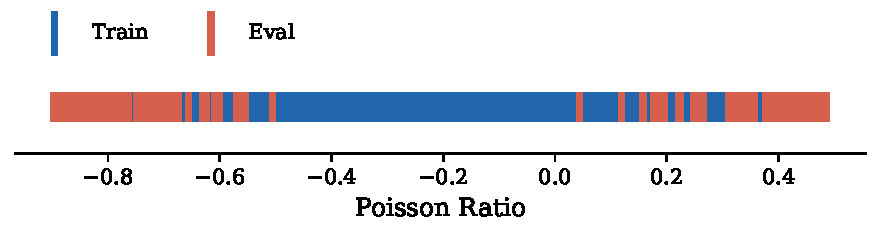
\includegraphics[width=\textwidth]{figures/split_visualization.pdf}
    \caption{Out-of-distribution evaluation split for the \texttt{Deforming Block OOD} environment. Each tick marks one task, colored by split assignment. Eval tasks are drawn from the tails of the Poisson ratio distribution, ensuring that evaluated material properties lie outside the training range.}
    \label{fig:ood_split}
\end{figure}

%
\subsection{Sheet Deformation.}
%
% \texttt{Sheet Deformation} consists of a $2$D sheet subjected to out-of-plane forces, resulting in $3$D deformations.
% The material is parameterized by Young's modulus, which is sampled log-uniformly from $[10, 500]$.
% The dataset contains $460/50/50$ train/val/test tasks, each with $16$ trajectories of $50$ simulation steps.
% In \texttt{Sheet Deformation}, a $2$D sheet is subjected to external forces perpendicular to the sheet, resulting in $3$D deformations. 
% The sheet's Young's Modulus is sampled log-uniformly from $[10, 500]$.
% Here, the dataset includes $460/50/50$ train/val/test tasks with $16$ trajectories of $50$ steps each.
%
This dataset considers the deformation of a thin square $2$D deformable sheet subjected to out-of-plane forces, resulting in $3$D deformations.
%
The sheet has initial stress-free edge length $l=140\;\text{mm}$. 
%
The thickness of the sheet is intrinsically defined as $t = 2.0 \;\text{mm}$. 
%
Nodes located at the outer edge of the sheet are clamped with zero displacement. The load is applied by two discrete external forces acting perpendicular to the thickness direction of the sheet. 
%
The force magnitude is fixed, while the normal force direction (upward or downward) and point of application are sampled uniformly.
%
To enable a continuous range of force application locations, the forces are applied uniformly to all nodes within a small radius  around the sampled application location. 
%
The forces are ramped up linearly from zero to their target magnitude over the simulated time. 
%
The material behavior of the sheet is modeled using isotropic linear elasticity with Young's modulus $E$ sampled log-uniformly in $[10, 500] \; \text{MPa}$ and Poisson's ratio $\nu{=}0.3$. 
%
The sheet is discretized using $225$ nodes and $392$ triangular elements. 
%
Geometric non-linearities due to large deformations are considered.
%
The simulation for the described environment is implemented in the finite element software \texttt{Abaqus/Standard} and solved using implicit time integration.
%
